\فصل{لیست‌}

\قسمت{مقدمه}
لیست‌ از جمله داده‌ساختارهای ساده و در عین حال بسیار مهم است. روش‌های مختلفی برای پیاده‌سازی این داده‌ساختار وجود دارد که هر یک از آنها دارای نقاط ضعف و قوت خود هستند. در این فصل پرسش‌های گوناگونی در مورد پیاده‌سازی‌های مختلف داده‌ساختار لیست بیان و به آنها پاسخ داده خواهد شد.

\قسمت{منابع مطالعاتی}
برای کسب اطلاعات بیشتر و مطالعه در مورد نوع داده‌ی انتزاعی لیست می‌توانید به فصل‌های چهارم {\cite{ebrahimi}} و {\cite{horowitz}} مراجعه کنید. برای آشنایی با لیست‌های پیوندی یکطرفه و دوطرفه فصل‌های چهارم {\cite{ebrahimi}} و {\cite{shaffer}} منابع مناسبی هستند. برای مطالعه درباره لیست‌های اندیسی می‌توانید به فصل دوم {\cite{aho}} رجوع کنید.

\قسمت{نوع داده‌ی انتزاعی لیست}

\سوال بدون در نظر گرفتن جزئیات مربوط به پیاده‌سازی داده‌ساختار لیست و به کمک توابع اولیه‌ی {\bcall{First}{}}،  {\bcall{Next}{}}، {\bcall{Delete}{}} و {\bcall{Retrieve}{}}، الگوریتمی بازگشتی بنویسید که با دریافت لیستی همچون {$L=\langle a_1,a_2,a_3,\ldots,a_n\rangle$} مقادیر آن را با ترتیب {$a_1,a_n,a_2,a_{n-1},\ldots$} چاپ کند و پس از چاپ مقدار هر عنصر آن عنصر را از لیست حذف کند. عملکرد توابع اولیه در ادامه آمده است.
\شروع{فقرات}
\فقره  {\bcall{First}{$L$}}: اشاره‌گر به عنصر اول لیست {$L$} را برمی‌گرداند. اگر لیست ورودی تهی باشد مقدار {\const{null}} به عنوان خروجی برگشت داده می‌شود.
\فقره  {\bcall{Last}{$L$}}: اشاره‌گر به عنصر آخر لیست {$L$} را برمی‌گرداند. در صورت تهی بودن لیست ورودی خروجی برابر با {\const{null}} خواهد بود.
\فقره {\bcall{Next}{$L,p$}}: اشاره‌گر به عنصری از لیست {$L$} که بعد از عنصری است که {$p$} به آن اشاره دارد را بازمی‌گرداند.
\فقره {\bcall{Delete}{$L,p$}}: عنصری که {$p$} به آن اشاره دارد را از لیست {$L$} حذف می‌کند. پس از انجام عمل حذف، {$p$} به عنصری که بعد از عنصر حذف شده قرار دارد اشاره خواهد کرد.
\فقره {\bcall{Retrieve}{$L,p$}}: مقدار داده‌ای عنصری از لیست {$L$} که اشاره‌گر {$p$} به آن اشاره دارد را برمی‌گرداند.
\پایان{فقرات}

\پاسخ

شبه کد زیربرنامه‌ی چاپ مقادیر یک لیست با ترتیب خواسته شده در صورت سوال، در الگوریتم {\eqref{ch3:alg:printList}} نشان داده شده است. روند کار این زیربرنامه بسیار ساده است. اگر لیست ورودی خالی باشد اجرای زیربرنامه خاتمه می‌یابد. در صورتی که لیست ورودی دارای تنها یک عنصر باشد آنگاه مقدار این عنصر به دست آمده و چاپ می‌شود. اگر لیست ورودی دارای بیش از یک عنصر باشد در این صورت ابتدا عنصر اول چاپ می‌شود، سپس عنصر آخر و در ادامه عناصر اول و آخر لیست حذف شده و زیربرنامه به صورت بازگشتی فراخوانی می‌شود تا سایر مقادیر لیست نیز چاپ شوند.

\begin{algorithm}
\caption{چاپ مقادیر یک لیست با ترتیبی خاص}\label{ch3:alg:printList}
\begin{latin}
\begin{algorithmic}[1]
\Procedure{PrintList}{$L$}
		\If{$L \isequal \const{null}$}
				\State	\Return
		\EndIf
		\If{$\bcall{First}{L} \isequal \bcall{Last}{L}$}
				\State	$f \gets \bcall{First}{L}$
				\State	$x \gets \bcall{Retrive}{L,f}$
				\State	\bcall{Write}{$x$}
		\Else
				\State	$f \gets \bcall{First}{L}$
				\State	$l \gets \bcall{Last}{L}$
				\State	$\id{xf} \gets \bcall{Retrieve}{L,f}$
				\State	$\id{xl} \gets \bcall{Retrieve}{L,l}$
				\State	\bcall{Write}{\id{xf}}				
				\State	\bcall{Write}{\id{xl}}
				\State	\bcall{Delete}{$L,f$}
				\State	\bcall{Delete}{$L,l$}				
				\State	\bcall{PrintList}{$L$}	
		\EndIf		
\EndProcedure	
\end{algorithmic}
\end{latin}
\end{algorithm}

\سوال الگوریتم {\eqref{ch3:alg:buggyDeleteElements}} قرار است تمام عناصری از یک لیست که دارای مقدار {$x$} هستند را از لیست حذف کند. توضیح دهید چرا این الگوریتم در مواقعی به درستی کار نمی‌کند. برای رفع مشکل باید چه تغییر یا تغییراتی در الگوریتم ایجاد کرد؟

\begin{algorithm}
\caption{حذف عناصر دارای مقدار {$x$} از یک لیست}\label{ch3:alg:buggyDeleteElements}
\begin{latin}
\begin{algorithmic}[1]
\Procedure{BuggyDeleteElements}{$L,x$}
	\State	$p \gets \bcall{First}{L}$
	\State	$q \gets \bcall{Last}{L}$	\label{ch3:alg:ln:buggyDelElemsLast}
	\While{$p \neq q$}\label{ch3:alg:ln:buggyDelElemsLoopBgn}
		\If{$\bcall{Retrieve}{L,p} \isequal x$}
			\State	$\bcall{Delete}{L,p}$
		\Else
			\State	$p \gets \bcall{Next}{L,p}$	
		\EndIf
	\EndWhile
\EndProcedure
\end{algorithmic}
\end{latin}
\end{algorithm}

\پاسخ

الگوریتم {\bcall{BuggyDeleteElements}{}} در حالتی که عنصر آخر لیست {$L$} دارای مقدار {$x$} باشد درست عمل نمی‌کند زیرا این عنصر باید از لیست حذف شود اما این اتفاق نمی‌افتد. دلیل حذف نشدن عنصر آخر این است که در الگوریتم مورد نظر هیچگاه مقدار عنصر آخر لیست بررسی نمی‌شود. برای اصلاح عملکرد الگوریتم باید خط  {\ref{ch3:alg:ln:buggyDelElemsLast}} را حذف کرده و در خط {\ref{ch3:alg:ln:buggyDelElemsLoopBgn}} به جای {$q$} از {\const{null}} استفاده کنیم. شبه کد الگوریتم اصلاح شده در قالب الگوریتم {\eqref{ch3:alg:deleteElements}} آورده شده است.

\begin{algorithm}
\caption{حذف عناصر دارای مقدار {$x$} از یک لیست}\label{ch3:alg:deleteElements}
\begin{latin}
\begin{algorithmic}[1]
\Procedure{DeleteElements}{$L,x$}
	\State	$p \gets \bcall{First}{L}$
	\While{$p \neq \const{null}$}
		\If{$\bcall{Retrieve}{L,p} \isequal x$}
			\State	$\bcall{Delete}{L,p}$
		\Else
			\State	$p \gets \bcall{Next}{L,p}$	
		\EndIf
	\EndWhile
\EndProcedure
\end{algorithmic}
\end{latin}
\end{algorithm}

\سوال لیست {$L$} دارای طول {$n$} است. اگر قطعه کدی که در ادامه آمده است را بر روی این لیست اعمال کنیم هر یک از توابع {\bcall{First}{}}، {\bcall{Last}{}} و {\bcall{Next}{}} چند بار اجرا می‌شوند؟

\begin{latin}
\begin{algorithmic}[1]
	\State	$p \gets \bcall{First}{L}$
	\While{$p \neq \bcall{Last}{L}$}
		\State	$q \gets p$
		\While{$q \neq \bcall{Last}{L}$}
			\State	$q \gets \bcall{Next}{L,q}$
			\State	$r \gets \bcall{First}{L}$
			\While{$r \neq q$}
				\State	$r \gets \bcall{Next}{L,r}$
			\EndWhile
		\EndWhile
		\State	$p \gets \bcall{Next}{L,p}$
	\EndWhile
\end{algorithmic}
\end{latin}

\پاسخ

ابتدا به سراغ به دست آوردن تعداد اجراهای تابع {\bcall{First}{}} می‌رویم. اگر تعداد تکرار حلقه میانی را به دست آوریم در واقع همان تعداد اجراهای تابع {\bcall{First}{}} را به دست آورده‌ایم زیرا با هر بار اجرای حلقه میانی تابع مورد نظر نیز یک بار اجرا می‌شود. حلقه بیرونی در مجموع {$n-1$} بار اجرا می‌شود. به ازای تکرار اول حلقه بیرونی حلقه میانی یک بار، به ازای تکرار دوم حلقه بیرونی حلقه میانی دو بار و به همین ترتیب تا تکرار {$n-1$} حلقه بیرونی که به ازای آن حلقه میانی نیز {$n-1$} بار اجرا می‌شود. با جمع مقادیر از یک تا {$n-1$} به این نتیجه می‌رسیم که حلقه میانی در مجموع {$n(n-1)/2$} بار اجرا می‌شود. چون در خط اول قطعه کد مورد نظر نیز یک بار تابع {\bcall{First}{}} اجرا می‌شود پس تعداد کل اجراهای تابع {\bcall{First}{}} برابر است با {$(n(n-1)/2)+1$}.

برای به دست آوردن تعداد اجراهای تابع {\bcall{Last}{}} باید دید سرآیند حلقه‌های بیرونی و میانی در مجموع چند بار اجرا می‌شوند زیرا با هر بار اجرای سرآیند یکی از این دو حلقه در واقع یک بار تابع {\bcall{Last}{}} اجرا می‌شود. جدول {\eqref{ch3:tbl:lastFunIters}} تعداد اجراهای سرآیند حلقه‌های بیرونی و میانی را به ازای مقادیر مختلف طول لیست ورودی نشان می‌دهد. با توجه به جدول {\eqref{ch3:tbl:lastFunIters}} مجموع تعداد اجراهای سرآیندهای حلقه درونی و میانی برابر است با {$n+(n(n+1)/2)-1$} و این رابطه برای هر {$n>0$} برقرار است. به این ترتیب اگر تعداد اجراهای تابع {\bcall{Last}{}} بر روی لیستی به طول {$n$} را با {$f(n)$} نشان دهیم آنگاه داریم:
\begin{displaymath}
f(n)=
\begin{cases}
1 & n=0\\
n+\dfrac{n(n+1)}{2}-1 & n>0
\end{cases}
\end{displaymath}

\begin{table}
\begin{center}
\small
\begin{tabular}{ccc}
\toprule[0.9pt]
\متن‌سیاه{تعداد اجرای سرآیند حلقه میانی} & \متن‌سیاه{تعداد اجرای سرآیند حلقه بیرونی} &  \متن‌سیاه{طول لیست}\\
\toprule[0.6pt]
$0$ & $1$ & $0$\\
$0$ & $1$ & $1$\\
$2$ & $2$ & $2$\\
$5$ & $3$ & $3$\\
$9$ & $4$ & $4$\\
$\vdots$ & $\vdots$ & $\vdots$\\
$\dfrac{n(n+1)}{2}-1$ & $n$ & $n$\\
\bottomrule[0.9pt]
\end{tabular}
\end{center}
\caption{تعداد اجراهای تابع {\lr{\textsc{Last}}} به ازای مقادیر مختلف طول لیست}\label{ch3:tbl:lastFunIters}
\end{table}

تعداد اجراهای تابع {\bcall{Next}{}} برابر با مجموع تعداد تکرار هر سه حلقه است زیرا با هر تکرار یکی از این حلقه‌ها یک بار تابع {\bcall{Next}{}} نیز اجرا می‌شود. جدول {\eqref{ch3:tbl:nextFunIters}} تعداد اجراهای حلقه‌های بیرونی، میانی و درونی را به ازای مقادیر مختلف طول لیست ورودی نشان می‌دهد. با توجه به جدول {\eqref{ch3:tbl:nextFunIters}} می‌توان گفت مجموع تعداد تکرار هر سه حلقه برابر است با:
\begin{equation}
(n-1) + \frac{n(n-1)}{2} + \left(\frac{n(n+1)(2n+1)}{6} - n^2\right)\label{ch3:eqn:nextFunIters}
\end{equation}
عبارت {\eqref{ch3:eqn:nextFunIters}} برای هر {$n>0$} برقرار است. به این ترتیب اگر {$g(n)$} را برابر با تعداد اجراهای تابع {\bcall{Next}{}} بر روی لیستی به طول {$n$} در نظر بگیریم خواهیم داشت:
\begin{displaymath}
g(n)=
\begin{cases}
0 & n=0\\
(n-1) + \dfrac{n(n-1)}{2} + \left(\dfrac{n(n+1)(2n+1)}{6} - n^2\right) & n>0
\end{cases}
\end{displaymath}

\begin{table}
\begin{center}
\small
\begin{tabular}{cccc}
\toprule[0.9pt]
\متن‌سیاه{تعداد اجرای حلقه درونی} & \متن‌سیاه{تعداد اجرای حلقه میانی} & \متن‌سیاه{تعداد اجرای حلقه بیرونی} &  \متن‌سیاه{طول لیست}\\
\toprule[0.6pt]
$0$ & $0$ & $0$ & $0$\\
$0$ & $0$ & $0$ & $1$\\
$1$ & $1$ & $1$ & $2$\\
$5$ & $3$ & $2$ & $3$\\
$14$ & $6$ & $3$ & $4$\\
$\vdots$ & $\vdots$ & $\vdots$ & $\vdots$\\
$\dfrac{n(n+1)(2n+1)}{6}-n^2$ & $\dfrac{n(n-1)}{2}$ & $n-1$ & $n$\\
\bottomrule[0.9pt]
\end{tabular}
\end{center}
\caption{تعداد اجراهای تابع {\lr{\textsc{Next}}} به ازای مقادیر مختلف طول لیست}\label{ch3:tbl:nextFunIters}
\end{table}

\قسمت{لیست‌ پیوندی یکطرفه}

\سوال زیربرنامه‌ای با نام {\bcall{MakeNull}{}} را در نظر بگیرید که از آن برای حذف تمامی عناصر یک لیست پیوندی یکطرفه استفاده می‌شود. این زیربرنامه را می‌توان به صورت بازگشتی یا غیربازگشتی نوشت. نسخه‌ی غیربازگشتی این زیربرنامه در الگوریتم {\eqref{ch3:alg:mkNull}} و نسخه‌ی بازگشتی در الگوریتم {\eqref{ch3:alg:recMkNull}} نشان داده شده است. با در نظر گرفتن پیاده‌سازی بازگشتی و غیربازگشتی زیربرنامه {\bcall{MakeNull}{}}، چه تفاوتی در ترتیب آزاد شدن فضای مصرفی عناصر لیست {$L$} در این دو زیربرنامه وجود دارد؟ نسخه‌ی بازگشتی زیربرنامه را به گونه‌ای تغییر دهید که از نظر آزادسازی فضای مصرفی لیست {$L$} همانند نسخه‌ی غیربازگشتی عمل کند.

\begin{algorithm}
\caption{حذف تمامی عناصر یک لیست پیوندی یکطرفه به صورت غیربازگشتی}\label{ch3:alg:mkNull}
\begin{latin}
\begin{algorithmic}[1]
\Procedure{MakeNull}{$L$}
		\While{$L \neq \const{null}$}
				\State	$p \gets L$
				\State	$L \gets \attrib{L}{next}$
				\State	\bcall{Free}{$p$}
		\EndWhile
\EndProcedure
\end{algorithmic}
\end{latin}
\end{algorithm}

\begin{algorithm}
\caption{حذف تمامی عناصر یک لیست پیوندی یکطرفه به صورت بازگشتی}\label{ch3:alg:recMkNull}
\begin{latin}
\begin{algorithmic}[1]
\Procedure{MakeNull}{$L$}
		\If{$L \isequal \const{null}$}
				\State \Return
		\Else
				\State	\bcall{MakeNull}{$\attrib{L}{next}$}
				\State	\bcall{Free}{$L$}
		\EndIf
\EndProcedure
\end{algorithmic}
\end{latin}
\end{algorithm}

\پاسخ

در نسخه‌ی غیر بازگشتی عناصر لیست از ابتدای لیست شروع به حذف شدن می‌کنند در حالی که در نسخه بازگشتی عناصر از انتها شروع به حذف شدن می‌کنند. به بیان بهتر ترتیب حذف عناصر در دو پیاده‌سازی برعکس یکدیگر است.

می‌توان نسخه‌ی بازگشتی را به صورتی بازنویسی کرد که عناصر از ابتدای لیست شروع به حذف شدن کنند. شبه ‌کد تغییر یافته‌ی نسخه  بازگشتی زیربرنامه {\bcall{MakeNull}{}} در الگوریتم {\eqref{ch3:alg:modRecMkNull}} آمده است.

\begin{algorithm}
\caption{حذف تمامی عناصر یک لیست پیوندی یکطرفه به صورت بازگشتی (تغییر یافته)}\label{ch3:alg:modRecMkNull}
\begin{latin}
\begin{algorithmic}[1]
\Procedure{MakeNull}{$L$}
		\If{$L \isequal \const{null}$}
				\State \Return
		\EndIf
		\State	$p \gets L$
		\State	$L \gets \attrib{L}{next}$
		\State	\bcall{Free}{$p$}			
		\State	\bcall{MakeNull}{$L$}
\EndProcedure
\end{algorithmic}
\end{latin}
\end{algorithm}

\سوال برای ایجاد یک کپی از یک لیست پیوندی یکطرفه به صورت بازگشتی، می‌توان از الگوریتم {\eqref{ch3:alg:recCopyList}} استفاده کرد. یک تابع غیربازگشتی برای کپی کردن یک لیست پیوندی یکطرفه بنویسید. در نسخه‌ی غیربازگشتی ممکن است تفاوت‌هایی در ایجاد سلول‌ها، اتصال آن‌ها به یکدیگر و ... نسبت به نسخه‌ی بازگشتی وجود داشته باشد. این تفاوت‌ها را ذکر کنید.

\begin{algorithm}
\caption{کپی یک لیست پیوندی یکطرفه به صورت بازگشتی}\label{ch3:alg:recCopyList}
\begin{latin}
\begin{algorithmic}[1]
\Function{CopyList}{$L$}
		\If{$L \isequal \const{null}$}
				\State \Return \const{null}
		\EndIf
		\State	\bcall{New}{$p$}
		\State	$\attrib{p}{data} \gets \attrib{L}{data}$
		\State	$\attrib{p}{next} \gets \bcall{Copy}{\attrib{L}{next}}$
		\State	\Return $p$
\EndFunction
\end{algorithmic}
\end{latin}
\end{algorithm}

\پاسخ

شبه کد نسخه‌ی غیربازگشتی تابع {\bcall{CopyList}{}} در الگوریتم {\eqref{ch3:alg:copyList}} نشان داده شده است.
\begin{algorithm}
\caption{کپی یک لیست پیوندی یکطرفه به صورت غیربازگشتی}\label{ch3:alg:copyList}
\begin{latin}
\begin{algorithmic}[1]
\Function{CopyList}{$L$}
		\If{$L \isequal \const{null}$}
				\State \Return \const{null}
		\EndIf
		\State	$p \gets L$
		\State	\bcall{New}{$t$}				
		\State	$q \gets t$
		\While{$ p \neq \const{null}$}
				\State	$\attrib{q}{data} \gets \attrib{p}{data}$
				\If{$\attrib{p}{next} \neq \const{null}}$
						\State	\bcall{New}{$\attrib{q}{next}$}												
						\State	$q \gets \attrib{q}{next}$
				\EndIf
				\State	$p \gets \attrib{p}{next}$
		\EndWhile
		\State	\Return $t$
\EndFunction
\end{algorithmic}
\end{latin}
\end{algorithm}

تفاوتی که نسخه‌ی غیربازگشتی تابع {\bcall{CopyList}{}} با نسخه‌ی بازگشتی خود دارد این است که ترتیب برقراری ارتباط سلول‌ها در نسخه‌ی بازگشتی از انتها به ابتدای لیست است در حالیکه در نسخه‌ی غیربازگشتی برقراری ارتباطات از ابتدا به انتهای لیست است. به بیان بهتر ترتیب انتساب مقادیر اشاره‌گر {\id{next}} در دو نسخه‌ی بازگشتی و غیربازگشتی متفاوت است.

\سوال یک لیست پیوندی یکطرفه‌ که دارای {$n$} عنصر است را در نظر بگیرید. فرض کنید عناصر این لیست را از ابتدا به انتها و به ترتیب از ۱ تا {$n$} شماره‌گذاری کرده‌ایم. تابعی به نام {\bcall{SplitList}{}} بنویسید که یک لیست پیوندی یکطرفه را دریافت و عناصر با شماره‌ی زوج را از آن حذف کرده و در لیست جدیدی درج کند. برای مثال اگر لیست ورودی به صورت شکل {\eqref{ch3:fig:splitListInputList}} باشد آنگاه پس از اجرای تابع باید به لیست‌های نشان داده شده در شکل {\eqref{ch3:fig:splitListOutputLists}} برسیم. (دقت داشته باشید که حذف عناصر از لیست ورودی و درج آنها در لیست جدید باید تنها با تغییر اشاره‌گرهای عناصر انجام شود و نباید هیچ گره‌‌ی جدیدی ایجاد شود).

\begin{figure}
\begin{center}
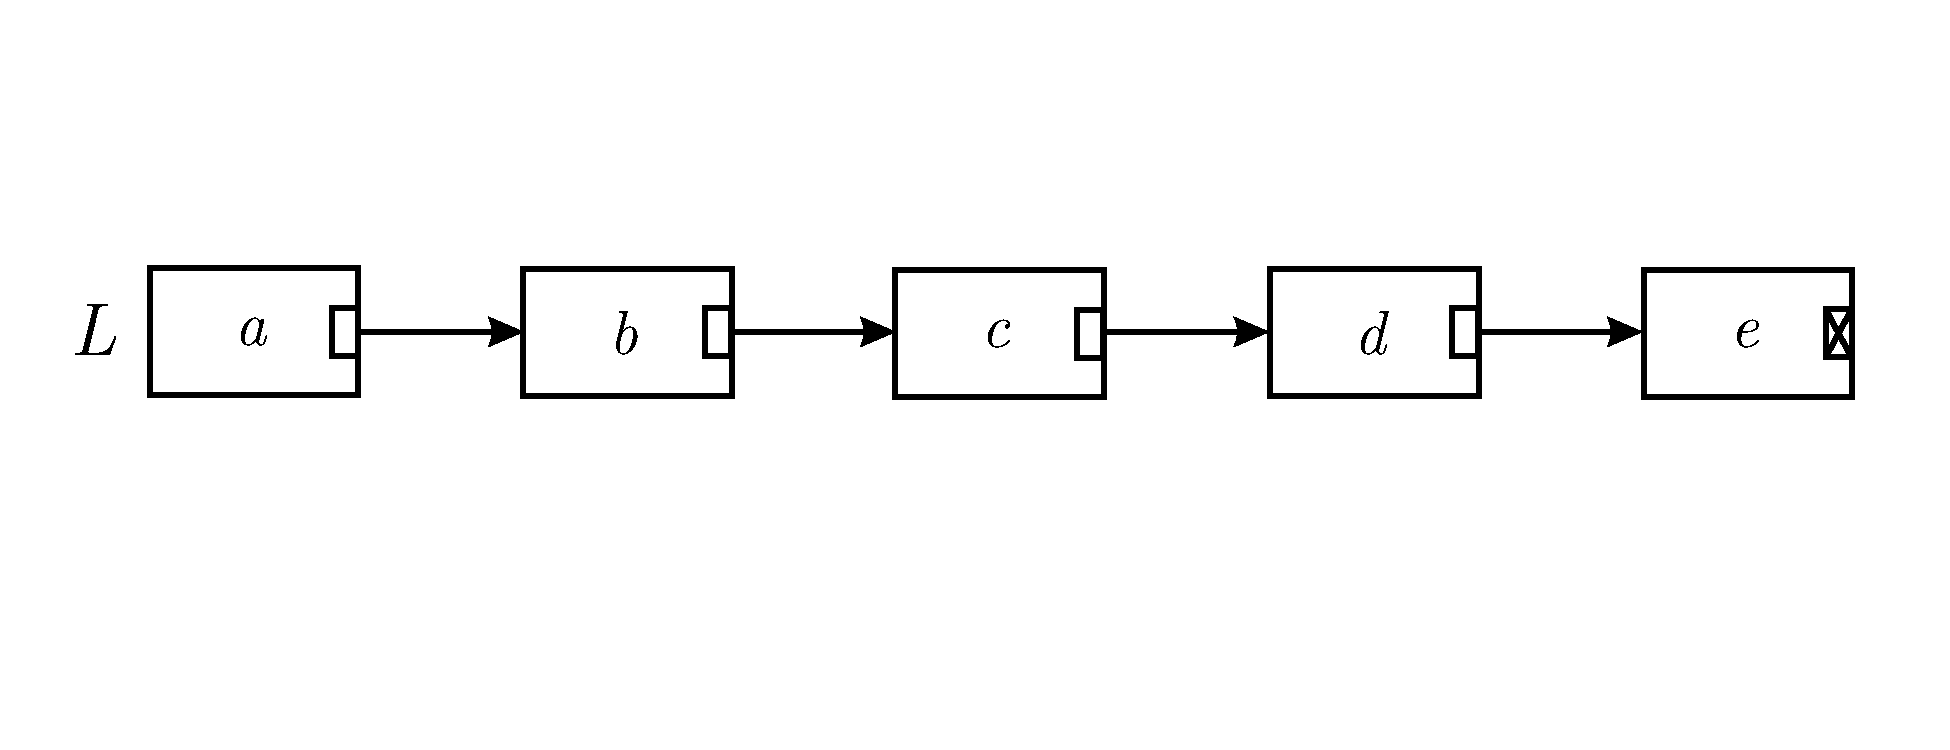
\includegraphics[scale=0.33]{figs/ch3/split_list_input_list.pdf}
\caption{یک لیست پیوندی نمونه به عنوان ورودی تابع {\lr{\textsc{SplitList}}}}\label{ch3:fig:splitListInputList}
\end{center}
\end{figure}

\begin{figure}
\begin{center}
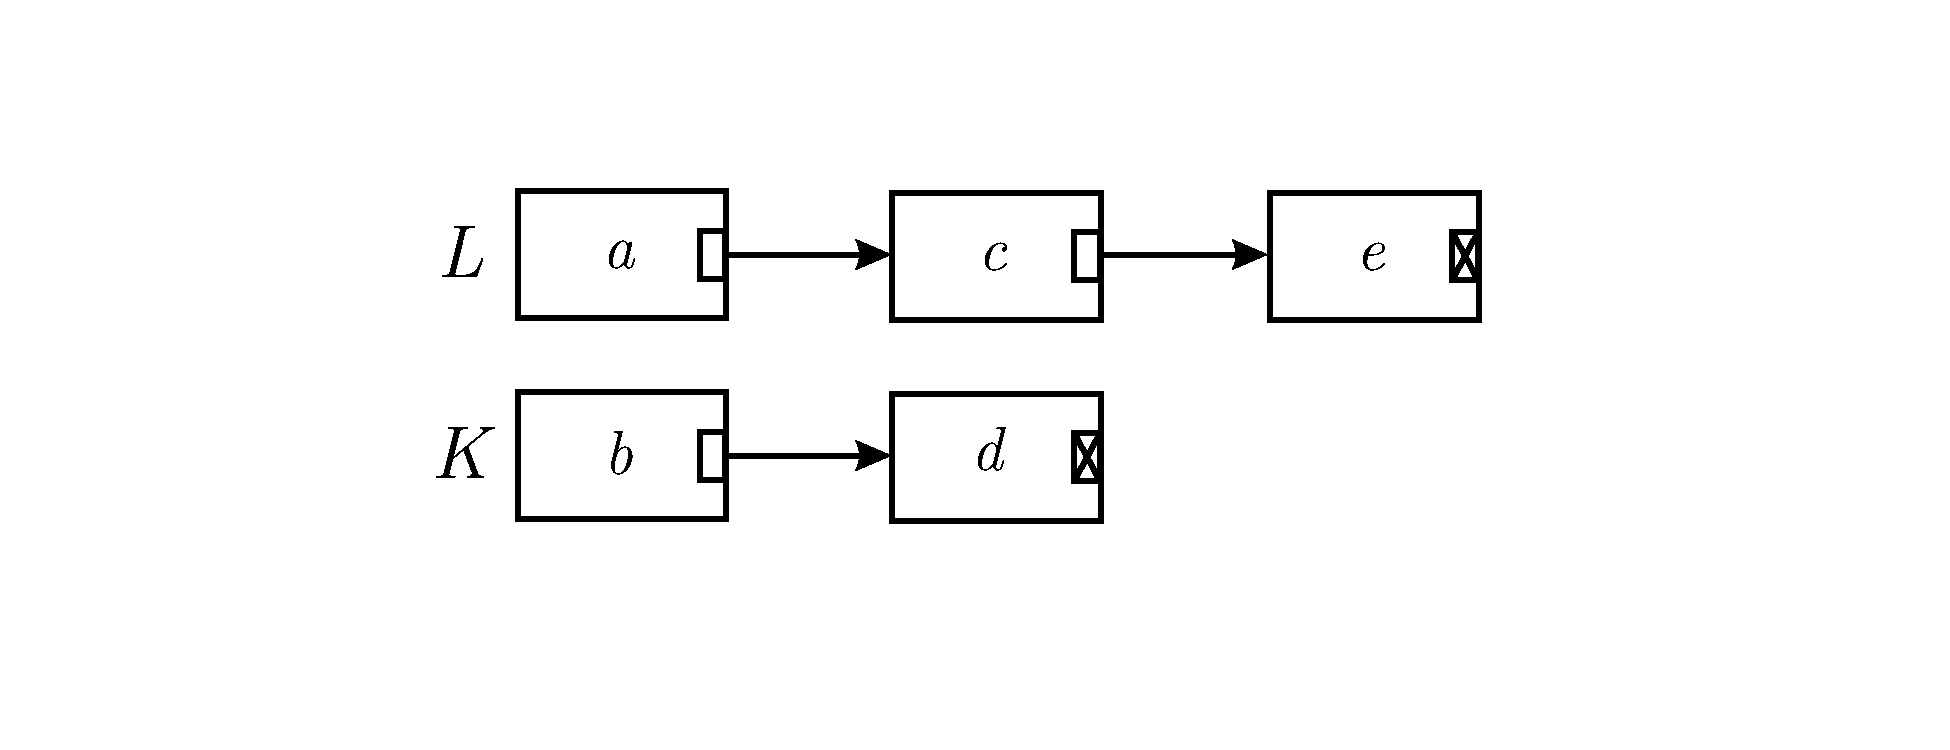
\includegraphics[scale=0.33]{figs/ch3/split_list_output_lists.pdf}
\caption{لیست‌های حاصل از اجرای تابع {\lr{\textsc{SplitList}}}}\label{ch3:fig:splitListOutputLists}
\end{center}
\end{figure}

\پاسخ

شبه کد الگوریتم جداسازی عناصر با شماره‌ی زوج از لیست ورودی در الگوریتم {\eqref{ch3:alg:split}} آمده است.
\begin{algorithm}
\caption{جداسازی عناصر با شماره‌ی زوج یک لیست پیوندی یکطرفه}\label{ch3:alg:split}
\begin{latin}
\begin{algorithmic}[1]
\Function{SplitList}{$L$}
		\If{$L \isequal \const{null} \Or \attrib{L}{next} \isequal \const{null}$}
				\State $K \gets \const{null}$
		\Else
				\State	$K \gets \attrib{L}{next}$
				\State	$\attrib{L}{next} \gets \attribb{L}{next}{next}$
				\State	$\attrib{K}{next} \gets $\bcall{SplitList}{$\attrib{L}{next}$}
		\EndIf
		\State	\Return $K$
\EndFunction
\end{algorithmic}
\end{latin}
\end{algorithm}

اگر لیست {$L$} تهی باشد آنگاه تنها کافیست لیست {$K$} را نیز برابر با تهی قرار دهیم. همچنین هنگامی که لیست {$L$} دارای تنها یک عنصر است  باید لیست {$K$} را برابر با تهی قرار دهیم زیرا در حالتی که فقط یک عنصر وجود دارد این عنصر دارای شماره یک است لیست {$L$} باید شامل آن عنصر بوده و لیست {$K$} تهی باشد.

اگر لیست {$L$} دارای بیش از یک عنصر باشد آنگاه ابتدا لیست {$K$} به عنصر دوم لیست {$L$} اشاره کرده و سپس عنصر بعد از عنصر اول در لیست {$L$} به عنصر سوم لیست {$L$} اشاره می‌کند. به این ترتیب {$L$} شامل عناصر با شماره‌های {$n ,\ldots , 4,3,1$}  و {$K$} شامل عنصر با شماره‌ی دو خواهد بود. سپس زیربرنامه‌ی {\bcall{SplitList}{}} به صورت بازگشتی  فراخوانی می‌شود تا به همین ترتیب عناصر با شماره‌ی فرد در لیست {$L$} و عناصر با شماره‌ی زوج در لیست {$K$} قرار بگیرند.

\سوال دو لیست پیوندی یکطرفه‌ی {\lr{L1}} و {\lr{L2}} را در نظر بگیرید. مقادیر موجود در این دو لیست به صورت صعودی مرتب هستند. تابعی غیربازگشتی به نام {\bcall{Merge}{}} بنویسید که تمام عناصر دو لیست {\lr{L1}} و {\lr{L2}} را در لیست جدید {\lr{L3}} درج کند به شکلی که عناصر لیست {\lr{L3}} نیز به صورت صعودی مرتب باشند. برای مثال اگر دو لیست نشان داده شده در شکل {\eqref{ch3:fig:mrgBefore}} به عنوان ورودی تابع {\bcall{Merge}{}} داده شوند آنگاه پس از پایان اجرای زیربرنامه باید به لیست جدیدی مانند آنچه در شکل {\eqref{ch3:fig:mrgAfter}} نمایش داده شده است برسیم.

\begin{figure}
\begin{center}
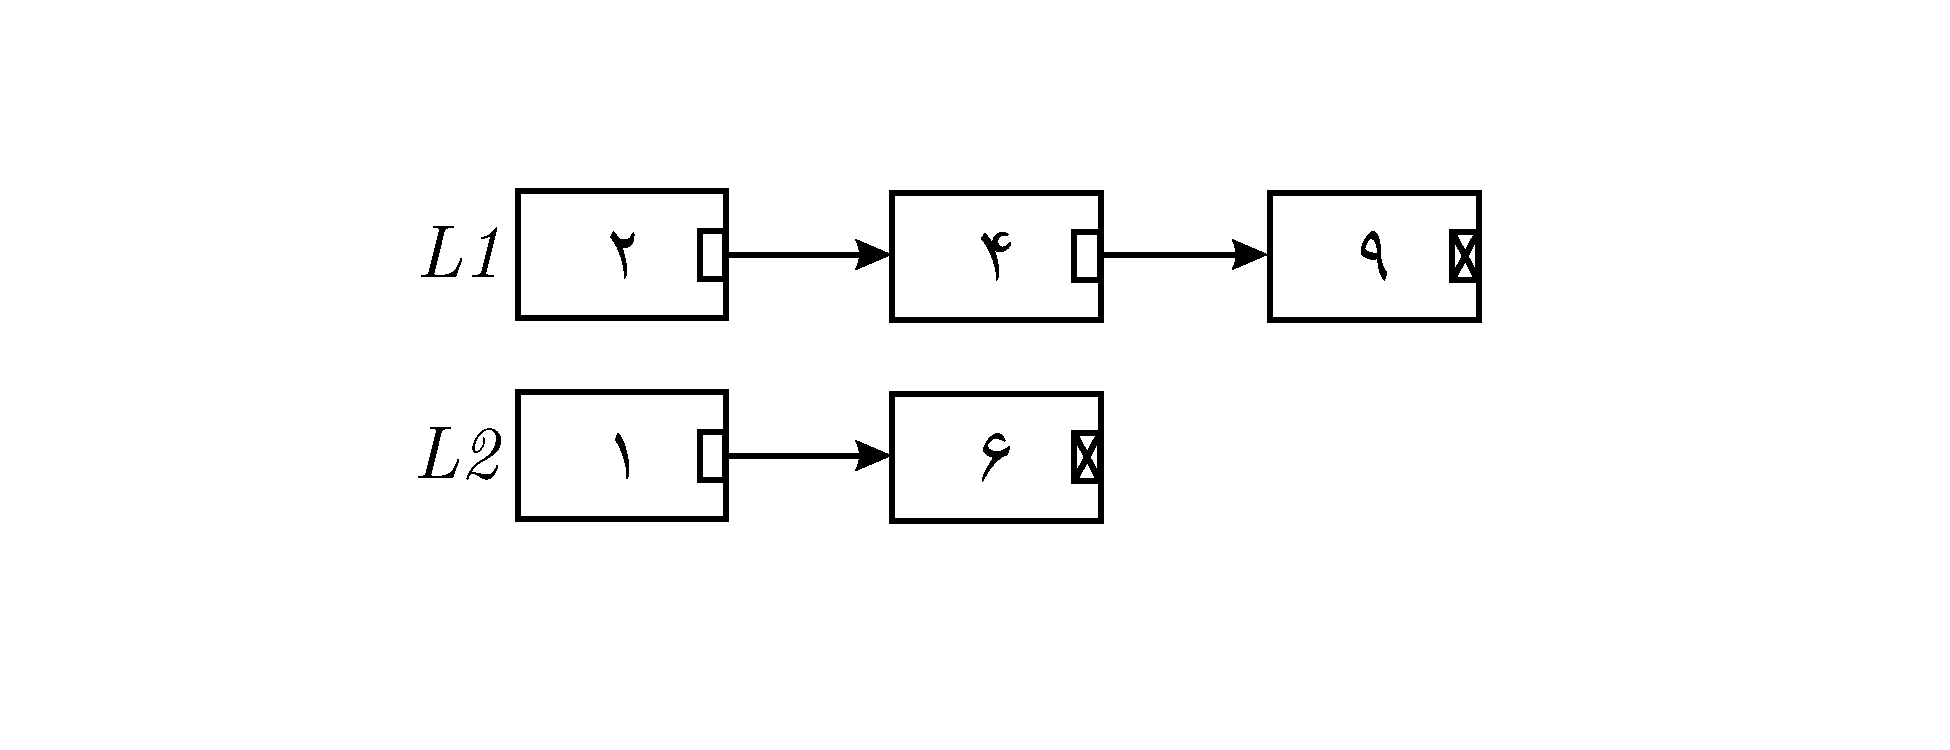
\includegraphics[scale=0.33]{figs/ch3/merge_input_lists.pdf}
\caption{دو لیست پیوندی نمونه به عنوان ورودی تابع {\lr{\textsc{Merge}}}}\label{ch3:fig:mrgBefore}
\end{center}
\end{figure}

\begin{figure}
\begin{center}
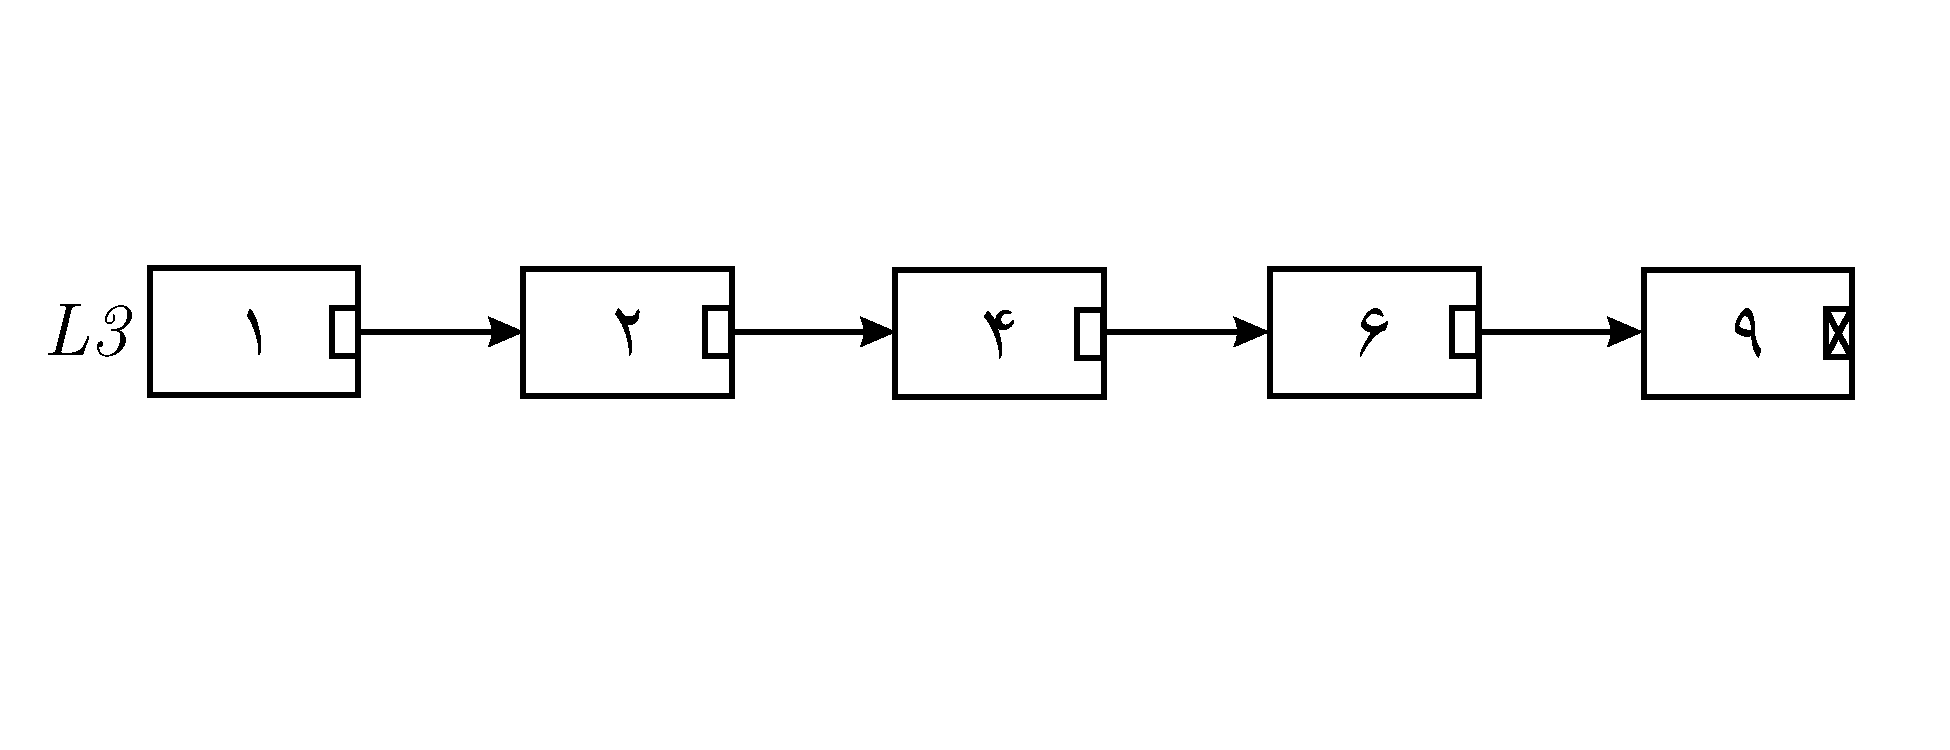
\includegraphics[scale=0.33]{figs/ch3/merge_output_list.pdf}
\caption{%
لیست پیوندی حاصل از اجرای تابع {\lr{\textsc{Merge}}} بر روی لیست‌های پیوندی شکل {\eqref{ch3:fig:mrgBefore}}
}
\label{ch3:fig:mrgAfter}
\end{center}
\end{figure}

\پاسخ

شبه کد تابع ادغام عناصر دو لیست پیوندی یکطرفه در الگوریتم {\eqref{ch3:alg:merge}} آورده شده است. بیان نحوه‌ی عملکرد این تابع در ادامه آمده است. 

\begin{algorithm}
\caption{ادغام عناصر دو لیست پیوندی یکطرفه}\label{ch3:alg:merge}
\begin{latin}
\begin{algorithmic}[1]
\Function{Merge}{$\id{L1},\id{L2}$}
			\State	\bcall{New}{$\id{L3}$}
			\State	$p \gets \id{L3}$		
			\State	$q \gets \id{L1}$
			\State	$r \gets \id{L2}$	
			\While{$q \neq \const{null} \And r \neq  \const{null}$}\label{ch3:alg:line:mrgWhileBegin}
					\State	\bcall{New}{$\attrib{p}{next}$}
					\If{$\attrib{q}{data} < \attrib{r}{data}$}
							\State	$\attrib{p}{data} \gets \attrib{q}{data}$
							\State	$q \gets \attrib{q}{next}$
					\Else
							\State	$\attrib{p}{data} \gets \attrib{r}{data}$
							\State	$r \gets \attrib{r}{next}$								
					\EndIf
					\State	$p \gets \attrib{p}{next}$
			\EndWhile\ \label{ch3:alg:line:mrgWhileEnd}
			\If{$q \isequal \const{null}$}\label{ch3:alg:line:mrgFirstIfBegin}
					\While{$r \neq \const{null}$}
							\State	$\attrib{p}{data} \gets \attrib{r}{data}$
							\If{$\attrib{r}{next} \neq \const{null}$}
									\State	\bcall{New}{$\attrib{p}{next}$}
									\State	$p \gets \attrib{p}{next}$
							\EndIf
							\State	$r \gets \attrib{r}{next}$
					\EndWhile
			\EndIf\ \label{ch3:alg:line:mrgFirstIfEnd}
			\If{$r \isequal \const{null}$}\label{ch3:alg:line:mrgSecIfBegin}
					\While{$q \neq \const{null}$}
							\State	$\attrib{p}{data} \gets \attrib{q}{data}$
							\If{$\attrib{q}{next} \neq \const{null}$}
									\State	\bcall{New}{$\attrib{p}{next}$}
									\State	$p \gets \attrib{p}{next}$
							\EndIf
							\State	$q \gets \attrib{q}{next}$
					\EndWhile
			\EndIf\ \label{ch3:alg:line:mrgSecIfEnd}	
		\State	\Return $\id{L3}$
\EndFunction
\end{algorithmic}
\end{latin}
\end{algorithm}

حلقه‌ی {\lr{while}} موجود در خطوط {\ref{ch3:alg:line:mrgWhileBegin}} تا {\ref{ch3:alg:line:mrgWhileEnd}} در هر دور از اجرای خود از میان دو عنصر جاری لیست‌های {\lr{L1}} و {\lr{L2}}، عنصری را که دارای مقدار کمتری است انتخاب کرده و در لیست {\lr{L3}} درج می‌کند. این حلقه زمانی پایان می‌یابد که حداقل یکی از دو لیست {\lr{L1}} یا {\lr{L2}} به انتهای خود برسند. پس از پایان اجرای حلقه باید بررسی شود که کدام لیست به انتهای خود رسیده است تا بتوان عناصر باقیمانده در لیست دیگر را در لیست {\lr{L3}} درج کرد. اگر لیست {\lr{L1}} به انتهای خود رسیده باشد باید عناصر باقیمانده در لیست {\lr{L2}} را به لیست {\lr{L3}} اضافه کرد (خطوط {\ref{ch3:alg:line:mrgFirstIfBegin}} تا {\ref{ch3:alg:line:mrgFirstIfEnd}}) و اگر لیست {\lr{L2}} به انتهای خود رسیده باشد آنگاه عناصر باقیمانده در لیست {\lr{L1}} باید در لیست {\lr{L3}} درج شوند (خطوط {\ref{ch3:alg:line:mrgSecIfBegin}} تا {\ref{ch3:alg:line:mrgSecIfEnd}}).

\سوال زیربرنامه‌ای غیربازگشتی بنویسید که عناصر تکراری یک لیست پیوندی یکطرفه را حذف کند. برای مثال اگر ورودی زیربرنامه لیست {$L=\langle a,b,a,c,b,d,d\rangle$} باشد آنگاه خروجی زیربرنامه باید لیست {$L=\langle a,b,c,d\rangle$} باشد. نسخه بازگشتی چنین زیربرنامه‌ای  را نیز طراحی کنید.

\پاسخ

شبه کد نسخه‌ی غیربازگشتی زیربرنامه‌ی حذف عناصر تکراری یک لیست پیوندی یکطرفه در قالب الگوریتم {\eqref{ch3:alg:rmvRedun}} نمایش داده شده است.
\begin{algorithm}
\caption{حذف عناصر با مقادیر تکراری از یک لیست پیوندی یکطرفه}\label{ch3:alg:rmvRedun}
\begin{latin}
\begin{algorithmic}[1]
\Procedure{RemoveRedundant}{$L$}
		\If{$L \isequal \const{null}$}
				\State	\Return
		\EndIf
		\State	$p \gets L$
		\While{$\attrib{p}{next} \neq \const{null}$}
				\State	$q \gets p$
				\While{$\attrib{q}{next} \neq \const{null}$}
						\If{$\attribb{q}{next}{data} \isequal \attrib{p}{data}$}
								\State	$r \gets \attrib{q}{next}$
								\State	$\attrib{q}{next} \gets \attrib{r}{next}$
								\State	\bcall{Free}{$r$}
						\Else
								\State	$q \gets \attrib{q}{next}$
						\EndIf
				\EndWhile
				\State	$p \gets \attrib{p}{next}$
		\EndWhile		
\EndProcedure
\end{algorithmic}
\end{latin}
\end{algorithm}

روش عملکرد زیربرنامه‌ی {\bcall{RemoveRedundant}{}} به این صورت است که در هر بار اجرای حلقه‌ی {\lr{while}} بیرونی، یک عنصر از لیست {$L$} که اشاره‌گر {$p$} به آن اشاره دارد به عنوان عنصر جاری در نظر گرفته می‌شود و عمل پیمایش در لیست {$L$}، از عنصر جاری به بعد، آغاز می‌شود. در حین انجام پیمایش اگر عنصری یافت شود که مقدار آن برابر با مقدار عنصر جاری باشد آنگاه این عنصر از لیست حذف می‌شود. اجرای حلقه‌ی {\lr{while}} بیرونی زمانی متوقف می‌شود که به ازای تمام عناصر لیست {$L$} عمل پیمایش انجام شده و تمام عناصر با مقادیر تکراری حذف شده باشند.

نسخه‌ی بازگشتی زیربرنامه‌ی حذف عناصر تکراری یک لیست پیوندی یکطرفه در الگوریتم {\eqref{ch3:alg:recRmvRedun}} آمده است. نسخه‌ی بازگشتی به این صورت عمل می‌کند که فرض می‌شود عنصر ابتدایی لیست وجود ندارد و زیربرنامه به صورت بازگشتی با شروع از عنصر دوم لیست ورودی فراخوانی می‌شود. پس از بازگشت از فراخوانی خط {\ref{ch3:alg:line:recCall}}، دارای لیستی خواهیم بود که ممکن است تعدادی از عناصر آن دارای مقدار یکسان با مقدار عنصر اول لیست باشند. به این ترتیب با شروع از ابتدای لیست و با انجام عمل پیمایش، هر عنصری که دارای مقدار یکسان با مقدار عنصر اول بود از لیست حذف می‌شود.
\begin{algorithm}
\caption{حذف عناصر با مقادیر تکراری از یک لیست پیوندی یکطرفه به صورت بازگشتی}\label{ch3:alg:recRmvRedun}
\begin{latin}
\begin{algorithmic}[1]
\Procedure{RemoveRedundant}{$L$}
		\If{$L \isequal \const{null} \Or \attrib{L}{next} \isequal \const{null}$}				
				\State	\Return
		\EndIf
		\State	\bcall{RemoveRedundant}{$\attrib{L}{next}$}\label{ch3:alg:line:recCall}
		\State	$p \gets L$
		\While{$\attrib{p}{next} \neq \const {null}$}
				\If{$\attribb{p}{next}{data} \isequal \attrib{L}{data}$}
						\State	$r \gets \attrib{p}{next}$
						\State	$\attrib{p}{next} \gets \attrib{r}{next}$
						\State	\bcall{Free}{$r$}
				\Else
						\State	$p \gets \attrib{p}{next}$
				\EndIf
		\EndWhile			
\EndProcedure
\end{algorithmic}
\end{latin}
\end{algorithm}

\سوال فرض کنید دارای یک لیست پیوندی یکطرفه به نام {$L$} و اشاره‌گر {$p$} هستیم. اشاره‌گر {$p$} به یکی از عناصر لیست {$L$} که عنصر آخر لیست نیست اشاره دارد. به جز اشاره‌گر {$p$} هیچ اشاره‌گر دیگری به هیچ یک از عناصر لیست {$L$} وجود ندارد مگر اینکه از ابتدای لیست پیمایش انجام شود. قطعه کدی از مرتبه‌ی {$O(1)$} بنویسید که مقدار موجود در عنصری که اشاره‌گر {$p$} به آن اشاره دارد را از لیست {$L$} حذف کند.

\پاسخ

تکه کد لازم برای حذف مقدار مورد نظر در ادامه آمده است.
\begin{latin}
\begin{algorithmic}[1]
		\State	$\attrib{p}{data} \gets \attribb{p}{next}{data}$
		\State	$t \gets \attrib{p}{next}$
		\State	$\attrib{p}{next} \gets \attribb{p}{next}{next}$
		\State	\bcall{Free}{$t$}
\end{algorithmic}
\end{latin}

\سوال فرض کنید از لیست پیوندی یکطرفه برای نگهداری اعداد صحیح مثبت استفاده شده است. روش ذخیره‌سازی یک عدد در چنین لیستی به این صورت است که رقم یکان در گره‌ی ابتدای لیست، رقم دهگان در گره‌ی دوم، رقم صدگان در گره‌ی سوم و به همین ترتیب تا رقم آخر که در گره‌ی آخر لیست قرار می‌گیرد. تابعی بنویسید که دو عدد صحیح، در قالب مطرح شده، را دریافت کرده و یک لیست پیوندی که حاوی حاصل جمع دو عدد ورودی است را بازگرداند.

\پاسخ

\قسمت{لیست‌ پیوندی دوطرفه}

\سوال لیست پیوندی دوطرفه {$L$} را در نظر بگیرید. گره‌ای مانند {$n$} در {$L$} دارای دو اشاره‌گر است که یکی به گره‌ی قبلی و دیگری به گره‌ی بعدی اشاره دارد (اشاره‌گرهای {\id{prev}} و {\id{next}}). با ترفندی خاص می‌توان لیست پیوندی دوطرفه {$L'$} را تنها با یک اشاره‌گر به ازای هر گره پیاده‌سازی کرد که در این صورت فضای مصرفی به ازای هر گره در یک لیست پیوندی دوطرفه برابر با گره‌ای در یک لیست پیوندی یکطرفه خواهد بود. این ترفند به این صورت است که هر گره مانند {$n'$} در {$L'$} دارای اشاره‌گری به نام {\id{np}} است. فرض کنید مقدار هر اشاره‌گر را می‌توان به صورت عددی {$k$} بیتی تفسیر کرد. به ازای هر گره مانند {$n$} در {$L$} گره‌ای مانند {$n'$} در {$L'$} در نظر می‌گیریم و قرار می‌دهیم {\lr{\attrib{n'}{np} $=$ \attrib{n}{\id{prev}} XOR \attrib{n}{\id{next}}} و همچنین 
{\lr{\attrib{n'}{\id{data}} $=$ \attrib{n}{\id{data}}}}.

با توجه به توضیحات ارائه شده الگوریتمی بنویسید که لیستی از نوع {$L'$}، مقدار {$x$} و اشاره‌گر {$p$} را دریافت کرده و گره‌ای با مقدار {$x$} را بعد از گره‌ای که {$p$} به آن اشاره دارد درج کند (مقدار {\const{Null}} را معادل با عدد صفر در نظر بگیرید).

\پاسخ

\قسمت{لیست‌ اندیسی}

\سوال پیاده‌سازی لیست توسط آرایه را در نظر بگیرید. زیربرنامه‌ای بنویسید که با در اختیار داشتن دو لیست {\lr{L1}} و {\lr{L2}}، عنصر با موقعیت {$p$} را از لیست {\lr{L1}} حذف کرده و در لیست {\lr{L2}} بعد از موقعیت {$q$} درج کند. سرآیند زیربرنامه نوشته شده  توسط شما باید به صورت زیر باشد:
\begin{latin}
\begin{algorithmic}[1]
\Statex	\bcall{Move}{$L1,p,L2,q$}
\end{algorithmic}
\end{latin}

\پاسخ

شبه کد حذف عنصر با موقعیت {$p$} از لیست {\lr{L1}} و درج آن بعد از موقعیت {$q$} در لیست {\lr{L2}} در قالب الگوریتم {\eqref{ch3:alg:move}} نمایش داده شده است. در این الگوریتم فرض شده است اگر مقدار {$q$} برابر با {\const{null}} باشد آنگاه عنصر حذف شده از لیست {\lr{L1}} باید در ابتدای لیست {\lr{L2}} درج شود.
\begin{algorithm}
\caption{حذف عنصری از لیستی اندیسی و درج آن در لیست اندیسی دیگر}\label{ch3:alg:move}
\begin{latin}
\begin{algorithmic}[1]
\Procedure{Move}{$\id{L1},p,\id{L2},q$}
		\If{$p \neq \id{L1}$}\label{ch3:alg:line:mvOutIfBegin}
				\State	$\id{temp} \gets \id{L1}$
				\While{$\attrib{space[temp]}{next} \neq p$}\label{ch3:alg:line:mvWhileBegin}
						\State	$\id{temp} \gets \attrib{space[temp]}{next}$
				\EndWhile\ \label{ch3:alg:line:mvWhileEnd}
				\If{$q \neq \const{null}$}\label{ch3:alg:mvInIf1Begin}
						\State	$\attrib{space[p]}{next} \gets \attrib{space[q]}{next}$
						\State	$\attrib{space[q]}{next} \gets p$
				\Else
						\State	$\attrib{space[p]}{next} \gets \id{L2}$
						\State	$\id{L2} \gets p$
				\EndIf\ \label{ch3:alg:line:mvOutIfEnd}
		\Else
				\If{$q \neq \const{null}$}\label{ch3:alg:line:mvOutElseBegin}
						\State	$\id{temp} \gets \attrib{space[\id{L1}]}{next}$
						\State	$\attrib{space[\id{L1}]}{next} \gets \id{L2}$
						\State	$\id{L2} \gets \id{L1}$
						\State	$\id{L1} \gets \id{temp}$
				\Else
						\State	$\id{temp} \gets \attrib{space[\id{L1}]}{next}$
						\State	$\attrib{space[\id{L1}]}{next} \gets \attrib{space[q]}{next}$
						\State	$\attrib{space[q]}{next} \gets \id{L1}$
						\State	$\id{L1} \gets \id{temp}$
				\EndIf
		\EndIf\ \label{ch3:alg:line:mvOutElseEnd}
\EndProcedure
\end{algorithmic}
\end{latin}
\end{algorithm}

در ادامه به توضیح روند کلی کار الگوریتم پرداخته می‌شود. عملکرد این الگوریتم، با توجه به اینکه اشاره‌گر {$p$} به کدام عنصر از لیست {\lr{L1}} اشاره می‌کند، به دو حالت تقسیم می‌شود. حالت اول در خطوط {\ref{ch3:alg:line:mvOutIfBegin}} تا {\ref{ch3:alg:line:mvOutIfEnd}} و حالت دوم در خطوط {\ref{ch3:alg:line:mvOutElseBegin}} تا {\ref{ch3:alg:line:mvOutElseEnd}} آمده است.

در حالت اول اشاره‌گر {$p$} به عنصری غیر از عنصر اول لیست {\lr{L1}} اشاره دارد. در این حالت باید در لیست {\lr{L1}} عمل پیمایش را انجام داد تا به عنصرِ قبل از عنصری برسیم که {$p$} به آن اشاره دارد (خطوط {\ref{ch3:alg:line:mvWhileBegin}} تا {\ref{ch3:alg:line:mvWhileEnd}}). سپس با توجه به اینکه اشاره‌گر {$q$} به ابتدای لیست {\lr{L2}} اشاره دارد یا خیر عملیات لازم برای درج عنصر در لیست {\lr{L2}} انجام می‌شود (خطوط {\ref{ch3:alg:mvInIf1Begin}} تا {\ref{ch3:alg:line:mvOutIfEnd}}).

در حالت دوم اشاره‌گر {$p$} به عنصر ابتدایی لیست {\lr{L1}} اشاره دارد. در این حالت نیازی به پیمایش لیست {\lr{L1}} وجود ندارد. تنها کافیست با توجه به اینکه اشاره‌گر {$q$} به ابتدای لیست {\lr{L2}} اشاره دارد یا خیر عملیات لازم برای حذف عنصر ابتدایی لیست {\lr{L1}} و درج آن در لیست {\lr{L2}} انجام شود (خطوط {\ref{ch3:alg:line:mvOutElseBegin}} تا {\ref{ch3:alg:line:mvOutElseEnd}}).

\سوال با فرض پیاده‌سازی لیست یک‌طرفه به کمک آرایه و در اختیار داشتن زیربرنامه‌های {\bcall{Dispose}{}} و {\bcall{Allocate}{}}، زیربرنامه‌های زیر را پیاده‌سازی کنید:
\شروع{فقرات}
\فقره {\bcall{Insert}{$L,p,d$}}: عنصری با مقدار {$d$} ساخته و آن را در لیست {$L$}، بعد از عنصری که {$p$} به آن اشاره دارد، درج می‌کند.
\فقره {\bcall{Delete}{$L,p$}}: عنصری که {$p$} به آن اشاره دارد را از لیست {$L$} حذف می‌کند.
\فقره {\bcall{Next}{$L,p$}}: اشاره‌گر به عنصری از لیست {$L$} که بعد از عنصری است که {$p$} به آن اشاره دارد را برمی‌گرداند.
\فقره {\bcall{Prev}{$L,p$}}: اشاره‌گر به عنصری از لیست {$L$} که قبل از عنصری است که {$p$} به آن اشاره دارد را برمی‌گرداند.
\پایان{فقرات}

\پاسخ

\سوال دانشگاهی با ۴۰۰۰ دانشجو و ۲۵۰۰ درس را در نظر بگیرید. این دانشگاه برای سیستم آموزشی خود قصد تولید دو نوع گزارش را دارد:
\شروع{شمارش}
\فقره گزارشی شامل افراد ثبت نام کننده برای هر درس به تفکیک درس.
\فقره گزارشی شامل دروس اخذ شده توسط هر دانشجو به تفکیک دانشجو.
\پایان{شمارش}
یک راه برای نگهداری اطلاعات مربوط به دانشجویان و کلاس‌ها استفاده از یک آرایه دو بعدی است. چنین آرایه‌ای دارای صد میلیون خانه خواهد بود! در این دانشگاه هر دانشجو به طور متوسط در سه درس ثبت نام می‌کند و این یعنی به طور متوسط تنها ۱۲۰ هزار خانه از این آرایه دارای مقادیر مفید هستند (حدود {$0.1$} درصد از کل فضای آرایه). در چنین حالتی فضای بسیار زیادی به هدر می‌رود. به کمک لیست‌های پیوندی داده‌ساختاری طراحی کنید که فقط شامل اطلاعات مفید باشد و همچنین مناسب تولید دو نوع گزارش ذکر شده هم باشد.

\پاسخ

شکل {\eqref{ch3:fig:custDS}} نمایش دهنده‌ی داده‌ساختار مورد نظر است. توجه داشته باشید که این داده‌ساختار تنها داده‌ساختار ممکن نیست. همانطور که از شکل مشخص است، چندین لیست پیوندی با یکدیگر ترکیب و در قالب یک لیست پیوندی پیچیده به نمایش درآمده‌اند. تمام لیست‌ها دارای گره‌ی سرلیست هستند و به صورت حلقوی پیاده‌سازی شده‌اند. روش به دست آوردن گزارش‌های ذکر شده در ادامه بیان خواهد شد.
\begin{figure}
\begin{center}
\scalebox{0.7} 
{
\begin{pspicture}(0,-4.23)(14.64,4.23)
\psdots[dotsize=0.14](4.42,3.25)
\psdots[dotsize=0.14](6.82,3.23)
\psdots[dotsize=0.14](9.22,3.25)
\psdots[dotsize=0.14](11.6,3.23)
\psframe[linewidth=0.04,dimen=outer](4.22,3.67)(3.02,2.83)
\psframe[linewidth=0.04,dimen=outer](4.6,3.67)(4.18,2.83)
\psframe[linewidth=0.04,dimen=outer](6.62,3.67)(5.42,2.83)
\psframe[linewidth=0.04,dimen=outer](7.0,3.67)(6.58,2.83)
\psframe[linewidth=0.04,dimen=outer](9.02,3.67)(7.82,2.83)
\psframe[linewidth=0.04,dimen=outer](9.4,3.67)(8.98,2.83)
\psframe[linewidth=0.04,dimen=outer](11.4,3.67)(10.2,2.83)
\psframe[linewidth=0.04,dimen=outer](11.78,3.67)(11.36,2.83)
\psframe[linewidth=0.04,dimen=outer](13.82,3.69)(12.62,2.85)
\psframe[linewidth=0.04,dimen=outer](14.2,3.69)(13.78,2.85)
\psline[linewidth=0.04cm,arrowsize=0.05291667cm 2.0,arrowlength=1.4,arrowinset=0.4]{->}(6.82,3.23)(6.8,0.53)
\psline[linewidth=0.04cm,arrowsize=0.05291667cm 2.0,arrowlength=1.4,arrowinset=0.4]{->}(9.22,3.25)(9.24,2.17)
\psline[linewidth=0.04cm,arrowsize=0.05291667cm 2.0,arrowlength=1.4,arrowinset=0.4]{->}(11.6,3.23)(11.58,2.17)
\usefont{T1}{ptm}{m}{n}
\rput(3.6403124,3.265){\large S1}
\rput(6.0915623,3.265){\large S2}
\rput(8.468281,3.265){\large S3}
\rput(10.835468,3.265){\large S4}
\rput(13.25375,3.265){\large S5}
\psframe[linewidth=0.04,dimen=outer](1.8,2.05)(0.6,1.21)
\psframe[linewidth=0.04,dimen=outer](2.18,2.05)(1.76,1.21)
\psframe[linewidth=0.04,dimen=outer](1.8,0.45)(0.6,-0.39)
\psframe[linewidth=0.04,dimen=outer](2.18,0.45)(1.76,-0.39)
\psframe[linewidth=0.04,dimen=outer](1.82,-1.15)(0.62,-1.99)
\psframe[linewidth=0.04,dimen=outer](2.2,-1.15)(1.78,-1.99)
\psframe[linewidth=0.04,dimen=outer](1.82,-2.75)(0.62,-3.59)
\psframe[linewidth=0.04,dimen=outer](2.2,-2.75)(1.78,-3.59)
\rput(1.2270312,1.625){\large C1}
\rput(1.2382812,0.025){\large C2}
\rput(1.235,-1.575){\large C3}
\rput(1.2621875,-3.155){\large C4}
\psline[linewidth=0.04cm,arrowsize=0.05291667cm 2.0,arrowlength=1.4,arrowinset=0.4]{->}(4.42,3.25)(4.42,2.15)
\psframe[linewidth=0.04,dimen=outer](9.4,2.05)(7.78,1.21)
\psline[linewidth=0.04cm](8.58,2.01)(8.58,1.25)
\psdots[dotsize=0.14](8.2,1.65)
\psdots[dotsize=0.14](8.98,1.65)
\psframe[linewidth=0.04,dimen=outer](4.62,2.05)(3.0,1.21)
\psline[linewidth=0.04cm](3.8,2.01)(3.8,1.25)
\psdots[dotsize=0.14](3.42,1.65)
\psdots[dotsize=0.14](4.2,1.65)
\psframe[linewidth=0.04,dimen=outer](11.82,2.07)(10.2,1.23)
\psline[linewidth=0.04cm](11.0,2.03)(11.0,1.27)
\psdots[dotsize=0.14](10.62,1.67)
\psdots[dotsize=0.14](11.4,1.67)
\psframe[linewidth=0.04,dimen=outer](7.02,0.45)(5.4,-0.39)
\psline[linewidth=0.04cm](6.2,0.41)(6.2,-0.35)
\psdots[dotsize=0.14](5.82,0.05)
\psdots[dotsize=0.14](6.6,0.05)
\psframe[linewidth=0.04,dimen=outer](14.22,0.47)(12.6,-0.37)
\psline[linewidth=0.04cm](13.4,0.43)(13.4,-0.33)
\psdots[dotsize=0.14](13.02,0.07)
\psdots[dotsize=0.14](13.8,0.07)
\psline[linewidth=0.04cm,arrowsize=0.05291667cm 2.0,arrowlength=1.4,arrowinset=0.4]{->}(3.42,1.63)(3.42,-1.15)
\psframe[linewidth=0.04,dimen=outer](9.4,-1.15)(7.78,-1.99)
\psline[linewidth=0.04cm](8.58,-1.19)(8.58,-1.95)
\psdots[dotsize=0.14](8.2,-1.55)
\psdots[dotsize=0.14](8.98,-1.55)
\psframe[linewidth=0.04,dimen=outer](4.62,-1.15)(3.0,-1.99)
\psline[linewidth=0.04cm](3.8,-1.19)(3.8,-1.95)
\psdots[dotsize=0.14](3.42,-1.55)
\psdots[dotsize=0.14](4.2,-1.55)
\psframe[linewidth=0.04,dimen=outer](11.82,-1.13)(10.2,-1.97)
\psline[linewidth=0.04cm](11.0,-1.17)(11.0,-1.93)
\psdots[dotsize=0.14](10.62,-1.53)
\psdots[dotsize=0.14](11.4,-1.53)
\psframe[linewidth=0.04,dimen=outer](14.22,-1.17)(12.6,-2.01)
\psline[linewidth=0.04cm](13.4,-1.21)(13.4,-1.97)
\psdots[dotsize=0.14](13.02,-1.57)
\psdots[dotsize=0.14](13.8,-1.57)
\psframe[linewidth=0.04,dimen=outer](7.0,-2.75)(5.38,-3.59)
\psline[linewidth=0.04cm](6.18,-2.79)(6.18,-3.55)
\psdots[dotsize=0.14](5.8,-3.15)
\psdots[dotsize=0.14](6.58,-3.15)
\psframe[linewidth=0.04,dimen=outer](11.82,-2.73)(10.2,-3.57)
\psline[linewidth=0.04cm](11.0,-2.77)(11.0,-3.53)
\psdots[dotsize=0.14](10.62,-3.13)
\psdots[dotsize=0.14](11.4,-3.13)
\psline[linewidth=0.04cm,arrowsize=0.05291667cm 2.0,arrowlength=1.4,arrowinset=0.4]{->}(8.2,1.65)(8.18,-1.11)
\psline[linewidth=0.04cm,arrowsize=0.05291667cm 2.0,arrowlength=1.4,arrowinset=0.4]{->}(10.62,1.67)(10.6,-1.09)
\psline[linewidth=0.04cm,arrowsize=0.05291667cm 2.0,arrowlength=1.4,arrowinset=0.4]{->}(14.0,3.25)(13.98,0.53)
\psdots[dotsize=0.14](14.0,3.23)
\psline[linewidth=0.04cm,arrowsize=0.05291667cm 2.0,arrowlength=1.4,arrowinset=0.4]{->}(5.82,0.05)(5.82,-2.71)
\psline[linewidth=0.04cm,arrowsize=0.05291667cm 2.0,arrowlength=1.4,arrowinset=0.4]{->}(13.02,0.05)(13.0,-1.11)
\psline[linewidth=0.04cm,arrowsize=0.05291667cm 2.0,arrowlength=1.4,arrowinset=0.4]{->}(10.62,-1.51)(10.62,-2.69)
\psline[linewidth=0.04cm](3.42,-1.57)(3.4,-4.21)
\psline[linewidth=0.04cm](3.38,-4.19)(2.62,-4.19)
\psline[linewidth=0.04cm](2.62,-4.17)(2.62,4.19)
\psline[linewidth=0.04cm](2.62,4.19)(3.8,4.19)
\psline[linewidth=0.04cm,arrowsize=0.05291667cm 2.0,arrowlength=1.4,arrowinset=0.4]{->}(3.8,4.19)(3.8,3.75)
\psline[linewidth=0.04cm](5.78,-3.17)(5.78,-4.17)
\psline[linewidth=0.04cm](5.02,-4.17)(5.02,4.19)
\psline[linewidth=0.04cm](5.02,4.19)(6.2,4.19)
\psline[linewidth=0.04cm,arrowsize=0.05291667cm 2.0,arrowlength=1.4,arrowinset=0.4]{->}(6.2,4.19)(6.2,3.75)
\psline[linewidth=0.04cm](5.02,-4.15)(5.76,-4.15)
\psline[linewidth=0.04cm](8.2,-1.55)(8.18,-4.19)
\psline[linewidth=0.04cm](8.16,-4.17)(7.42,-4.17)
\psline[linewidth=0.04cm](7.42,-4.15)(7.42,4.21)
\psline[linewidth=0.04cm](7.42,4.21)(8.6,4.21)
\psline[linewidth=0.04cm,arrowsize=0.05291667cm 2.0,arrowlength=1.4,arrowinset=0.4]{->}(8.6,4.21)(8.6,3.77)
\psline[linewidth=0.04cm](10.62,-3.17)(10.62,-4.17)
\psline[linewidth=0.04cm](9.84,-4.17)(9.84,4.19)
\psline[linewidth=0.04cm](9.84,4.19)(11.02,4.19)
\psline[linewidth=0.04cm,arrowsize=0.05291667cm 2.0,arrowlength=1.4,arrowinset=0.4]{->}(11.02,4.19)(11.02,3.75)
\psline[linewidth=0.04cm](9.84,-4.15)(10.64,-4.15)
\psline[linewidth=0.04cm](13.02,-1.57)(13.0,-4.21)
\psline[linewidth=0.04cm](13.02,-4.19)(12.24,-4.19)
\psline[linewidth=0.04cm](12.24,-4.17)(12.24,4.19)
\psline[linewidth=0.04cm](12.24,4.19)(13.42,4.19)
\psline[linewidth=0.04cm,arrowsize=0.05291667cm 2.0,arrowlength=1.4,arrowinset=0.4]{->}(13.42,4.19)(13.42,3.75)
\psdots[dotsize=0.14](2.0,1.61)
\psdots[dotsize=0.14](2.0,-0.01)
\psdots[dotsize=0.14](2.0,-1.59)
\psdots[dotsize=0.14](2.0,-3.17)
\psline[linewidth=0.04cm,arrowsize=0.05291667cm 2.0,arrowlength=1.4,arrowinset=0.4]{->}(2.0,1.61)(2.98,1.61)
\psline[linewidth=0.04cm,arrowsize=0.05291667cm 2.0,arrowlength=1.4,arrowinset=0.4]{->}(2.02,-1.59)(2.98,-1.59)
\psline[linewidth=0.04cm,arrowsize=0.05291667cm 2.0,arrowlength=1.4,arrowinset=0.4]{->}(8.96,1.65)(10.16,1.63)
\psline[linewidth=0.04cm,arrowsize=0.05291667cm 2.0,arrowlength=1.4,arrowinset=0.4]{->}(8.98,-1.55)(10.18,-1.57)
\psline[linewidth=0.04cm,arrowsize=0.05291667cm 2.0,arrowlength=1.4,arrowinset=0.4]{->}(11.4,-1.53)(12.6,-1.55)
\psline[linewidth=0.04cm,arrowsize=0.05291667cm 2.0,arrowlength=1.4,arrowinset=0.4]{->}(4.18,1.65)(7.76,1.65)
\psline[linewidth=0.04cm,arrowsize=0.05291667cm 2.0,arrowlength=1.4,arrowinset=0.4]{->}(4.2,-1.55)(7.78,-1.55)
\psline[linewidth=0.04cm,arrowsize=0.05291667cm 2.0,arrowlength=1.4,arrowinset=0.4]{->}(6.6,-3.15)(10.18,-3.15)
\psline[linewidth=0.04cm,arrowsize=0.05291667cm 2.0,arrowlength=1.4,arrowinset=0.4]{->}(1.96,-0.01)(5.36,-0.01)
\psline[linewidth=0.04cm,arrowsize=0.05291667cm 2.0,arrowlength=1.4,arrowinset=0.4]{->}(6.58,0.07)(12.58,0.03)
\psline[linewidth=0.04cm,arrowsize=0.05291667cm 2.0,arrowlength=1.4,arrowinset=0.4]{->}(2.04,-3.17)(5.36,-3.15)
\psline[linewidth=0.04cm](11.42,1.67)(14.58,1.67)
\psline[linewidth=0.04cm](14.6,1.67)(14.6,0.83)
\psline[linewidth=0.04cm](14.6,0.83)(0.0,0.81)
\psline[linewidth=0.04cm](0.02,0.83)(0.02,1.59)
\psline[linewidth=0.04cm,arrowsize=0.05291667cm 2.0,arrowlength=1.4,arrowinset=0.4]{->}(0.02,1.59)(0.5,1.59)
\psline[linewidth=0.04cm](14.6,0.07)(14.6,-0.77)
\psline[linewidth=0.04cm](14.6,-0.77)(0.0,-0.79)
\psline[linewidth=0.04cm](0.02,-0.77)(0.02,-0.01)
\psline[linewidth=0.04cm,arrowsize=0.05291667cm 2.0,arrowlength=1.4,arrowinset=0.4]{->}(0.02,-0.01)(0.5,-0.01)
\psline[linewidth=0.04cm](13.8,0.07)(14.6,0.05)
\psline[linewidth=0.04cm](14.62,-1.57)(14.62,-2.41)
\psline[linewidth=0.04cm](14.62,-2.41)(0.02,-2.43)
\psline[linewidth=0.04cm,arrowsize=0.05291667cm 2.0,arrowlength=1.4,arrowinset=0.4]{->}(0.04,-1.65)(0.52,-1.65)
\psline[linewidth=0.04cm](13.82,-1.57)(14.62,-1.59)
\psline[linewidth=0.04cm](0.02,-2.41)(0.02,-1.65)
\psline[linewidth=0.04cm](11.42,-3.13)(14.58,-3.13)
\psline[linewidth=0.04cm](14.6,-3.13)(14.6,-3.97)
\psline[linewidth=0.04cm](14.6,-3.97)(0.0,-3.99)
\psline[linewidth=0.04cm](0.02,-3.97)(0.02,-3.21)
\psline[linewidth=0.04cm,arrowsize=0.05291667cm 2.0,arrowlength=1.4,arrowinset=0.4]{->}(0.02,-3.21)(0.5,-3.21)
\end{pspicture} 
}
\caption{}\label{ch3:fig:custDS}
\end{center}
\end{figure}

برای استخراج اسامی افراد ثبت‌نام کننده در یک کلاس، مثلاً کلاس {\lr{C3}} ، کافیست از گره با سرلیست {\lr{C3}} شروع کرده و به سمت راست این لیست حرکت کنیم. بعد از رفتن به اولین گره از لیست {\lr{C3}} ، مقدار جاری اشاره‌گر را ذخیره می‌کنیم و سپس با استفاده از اشاره‌گر به سمتِ پایین این گره به صورت عمودی در لیست حرکت کرده تا به سرلیست لیست عمودی برسیم (در اینجا لیست {\lr{S1}}). به این ترتیب نام اولین دانشجو ثبت نام کننده در کلاس {\lr{C3}} به دست می‌‌آید. در گام بعد و برای به دست آوردن نام دانشجوی بعدی از اشاره‌گر ذخیره شده در گام قبل استفاده کرده و دوباره به سمت راست در لیست {\lr{C3}} حرکت کرده و روند حرکت عمودی در ساختمان داده را ادامه می‌دهیم. به این ترتیب می‌توان اسامی تمام افراد ثبت نام کننده در یک کلاس را به دست آورد.

برای به دست آوردن دروس ثبت نام شده توسط یک دانشجو به روشی مشابه با پاراگراف قبل عمل می‌کنیم با این تفاوت که در اینجا از گره با سر لیست حاوی نام دانشجو شروع کرده و به سمت پایین لیست حرکت می‌کنیم و برای یافتن هر درس به صورت افقی لیست‌ها را پیمایش می‌کنیم.